\documentclass{article}
\usepackage{ctex}
\usepackage[xcolor]{listings} % 导入代码高亮包
\usepackage{xcolor} % 导入颜色包
\usepackage{graphicx} % 导入图形包
\usepackage[margin=1in]{geometry} % 调整页边距
\author{陈祎伟\\3230102357}
\title{Lab 4 : L1 Cache 设计}
\date{2025年4月16日}

\lstset{
    basicstyle=\ttfamily\footnotesize, % 基本样式,小号等宽字体
    numbers=left,                      % 行号位置
    numberstyle=\tiny\color{gray},     % 行号样式
    stepnumber=1,                      % 行号步长
    numbersep=5pt,                     % 行号与代码间距
    backgroundcolor=\color{white},     % 代码背景色
    showspaces=false,                  % 显示空格
    showstringspaces=false,            % 显示字符串中的空格
    showtabs=false,                    % 显示制表符
    frame=single,                      % 代码框
    rulecolor=\color{black},           % 框颜色
    tabsize=4,                         % 制表符宽度
    captionpos=b,                      % 标题位置
    breaklines=true,                   % 自动换行
    breakatwhitespace=false,           % 仅在空格处换行
    title=\lstname,                    % 显示文件名
    keywordstyle=\color{blue},         % 关键字颜色
    commentstyle=\color{brown},        % 注释颜色
    stringstyle=\color{red},           % 字符串颜色
    escapeinside={\%*}{*)},            % 特殊字符
    morekeywords={*,...},              % 额外关键字
    language=[x86masm]Assembler        % 定义asm语言
}

\begin{document}
\maketitle
\section{设计思路}
\subsection{cache模块}
cache模块将可能的访存情况分为了4种:load, edit, store, invalid。\par
四种情况互不干涉,load是从cache中读取数据,edit是将cache中的数据进行修改,store是将数据写入cache,invalid是将cache中的数据置为无效。\par
为了正确实现 LRU 替换策略下的各种访存情况,使用如下信号进行控制:\par
    \begin{lstlisting}[language=Verilog]
    valid <= recent1 ? valid2 : valid1;
    dirty <= recent1 ? dirty2 : dirty1;
    tag <= recent1 ? tag2 : tag1;

    hit <= hit1 | hit2; 
    \end{lstlisting}

其中,前三个信号用于获取写入cache时,写入位置的相应状态信息;\par
而hit信号则用于判断cache是否命中。\par


\subsection{cmu模块}
cmu模块是cache的控制模块,主要用于控制cache的读写操作。\par
cmu分为5个状态:S\_IDLE, S\_PRE\_BACK, S\_BACK, S\_FILL, S\_WAIT。\par
各状态的相互转换如下:\par
\begin{itemize}
    \item S\_IDLE:空闲状态,等待访存请求。
    \begin{lstlisting}[language=Verilog]
    S_IDLE: begin
        if (en_r || en_w) begin
            if (cache_hit)
                next_state = S_IDLE;
            else if (cache_valid && cache_dirty)
                next_state = S_PRE_BACK;
            else
                next_state = S_FILL;
        end
        next_word_count = 2'b00;
    end
    \end{lstlisting}
    下一个状态由访存请求的类型决定:\par
    当 hit 时,不需要进行对内存的读写操作,直接进入空闲状态;\par
    当 miss 时,若数据为 dirty,则需要将数据写回内存,进入 S\_PRE\_BACK 状态,否则进入 S\_FILL 状态。\par

    \item S\_PRE\_BACK:写回内存准备状态,先对 cache 进行一次读操作,\par
    \begin{lstlisting}[language=Verilog]
    S_PRE_BACK: begin
        next_state = S_BACK;
        next_word_count = 2'b00;
    end
    \end{lstlisting}
    进入 S\_BACK 状态,准备将数据写回内存。\par

    \item S\_BACK:写回内存状态,进行数据的写回操作。\par
    \begin{lstlisting}[language=Verilog]
    S_BACK: begin
        if (mem_ack_i && word_count == {ELEMENT_WORDS_WIDTH{1'b1}})    // wrote back all words, 1 cache line = 4 words
            next_state = S_FILL;
        else
            next_state = S_BACK;

        if (mem_ack_i)
            next_word_count = word_count + 1'b1;
        else
            next_word_count = word_count;
    end
    \end{lstlisting}
    当收到内存的 ack 信号后,对已完成的 word 进行计数,\par
    当所有 word 都写回后,进入 S\_FILL 状态。\par
    否则,继续保持在 S\_BACK 状态。\par

    \item S\_FILL:填充状态,进行数据的填充操作。\par
    \begin{lstlisting}[language=Verilog]
    S_FILL: begin
        if (mem_ack_i && word_count == {ELEMENT_WORDS_WIDTH{1'b1}})
            next_state = S_WAIT;
        else
            next_state = S_FILL;

        if (mem_ack_i)
            next_word_count = word_count + 1'b1;
        else
            next_word_count = word_count;
    end
    \end{lstlisting}
    同样的,当收到内存的 ack 信号后,对已完成的 word 进行计数,\par
    当所有 word 都填充完成后,进入 S\_WAIT 状态。\par
    否则,继续保持在 S\_FILL 状态。\par

    \item S\_WAIT:执行之前由于 miss 而不能进行的 Cache 操作。\par
    \begin{lstlisting}[language=Verilog]
    S_WAIT: begin
        next_state = S_IDLE;
        next_word_count = 2'b00;
    end
    \end{lstlisting}
    miss 消除后,可以正常进行读写操作,回到 S\_IDLE 状态。\par
\end{itemize}

此外,由于 cache miss 等带来的延迟,在一些情况下需要对 CPU 进行 stall,实现如下:\par
    \begin{lstlisting}[language=Verilog]
    assign stall = next_state != S_IDLE;
    \end{lstlisting}

\newpage
\section{思考题}
\subsection{在实验报告分别展示 Cache hit、Cache miss+dirty 两种情况,分析两种情况下的状态机状态变化以及需要的时钟周期。}
\begin{enumerate}
    \item Cache hit:\par
    \begin{figure}[h]
        \centering
        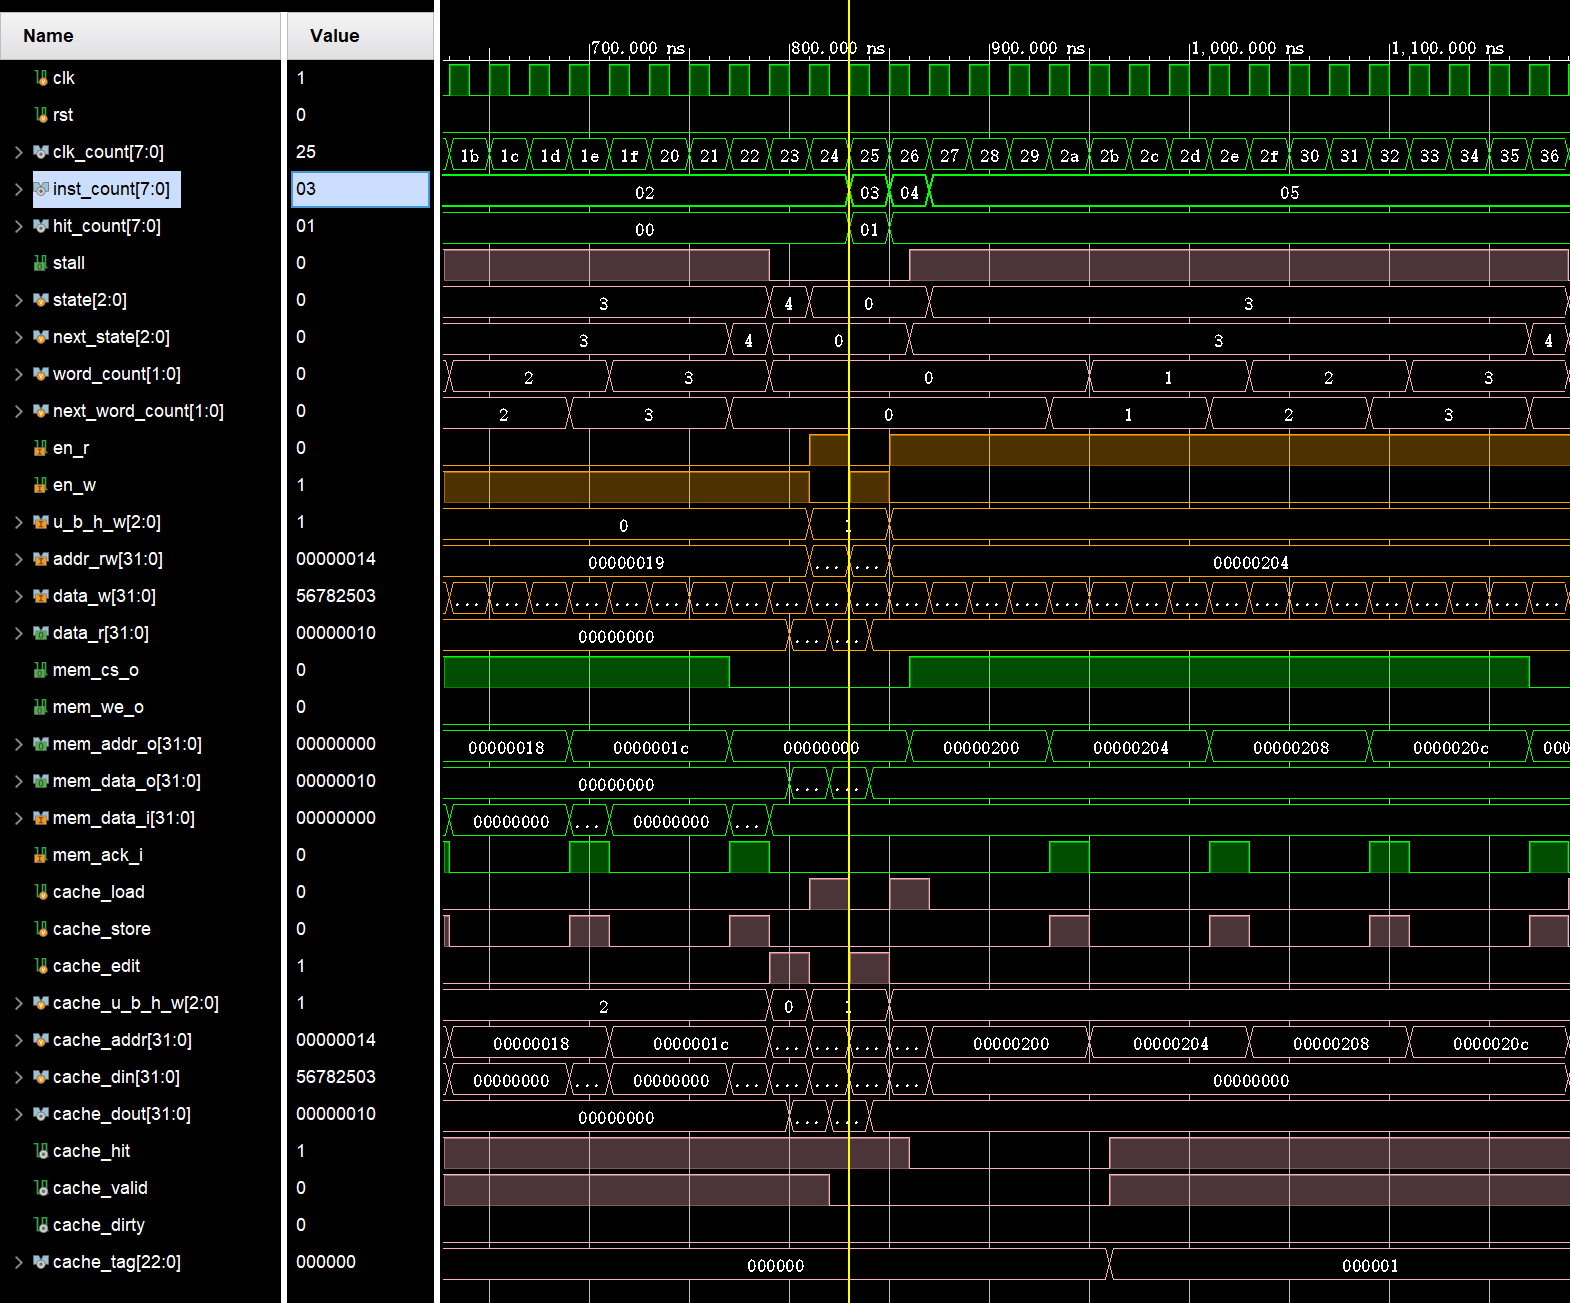
\includegraphics[width=1\textwidth]{images/cache_hit.png}
        \caption{Cache hit 仿真结果}
        \label{fig:cache_hit}
    \end{figure}
    当 cache 命中时,状态机的状态变化一直保持在 S\_IDLE 状态,只需要一个时钟周期即可完成读写操作。\par
    
    \newpage
    \item Cache miss + dirty:\par
    \begin{figure}[h]
        \centering
        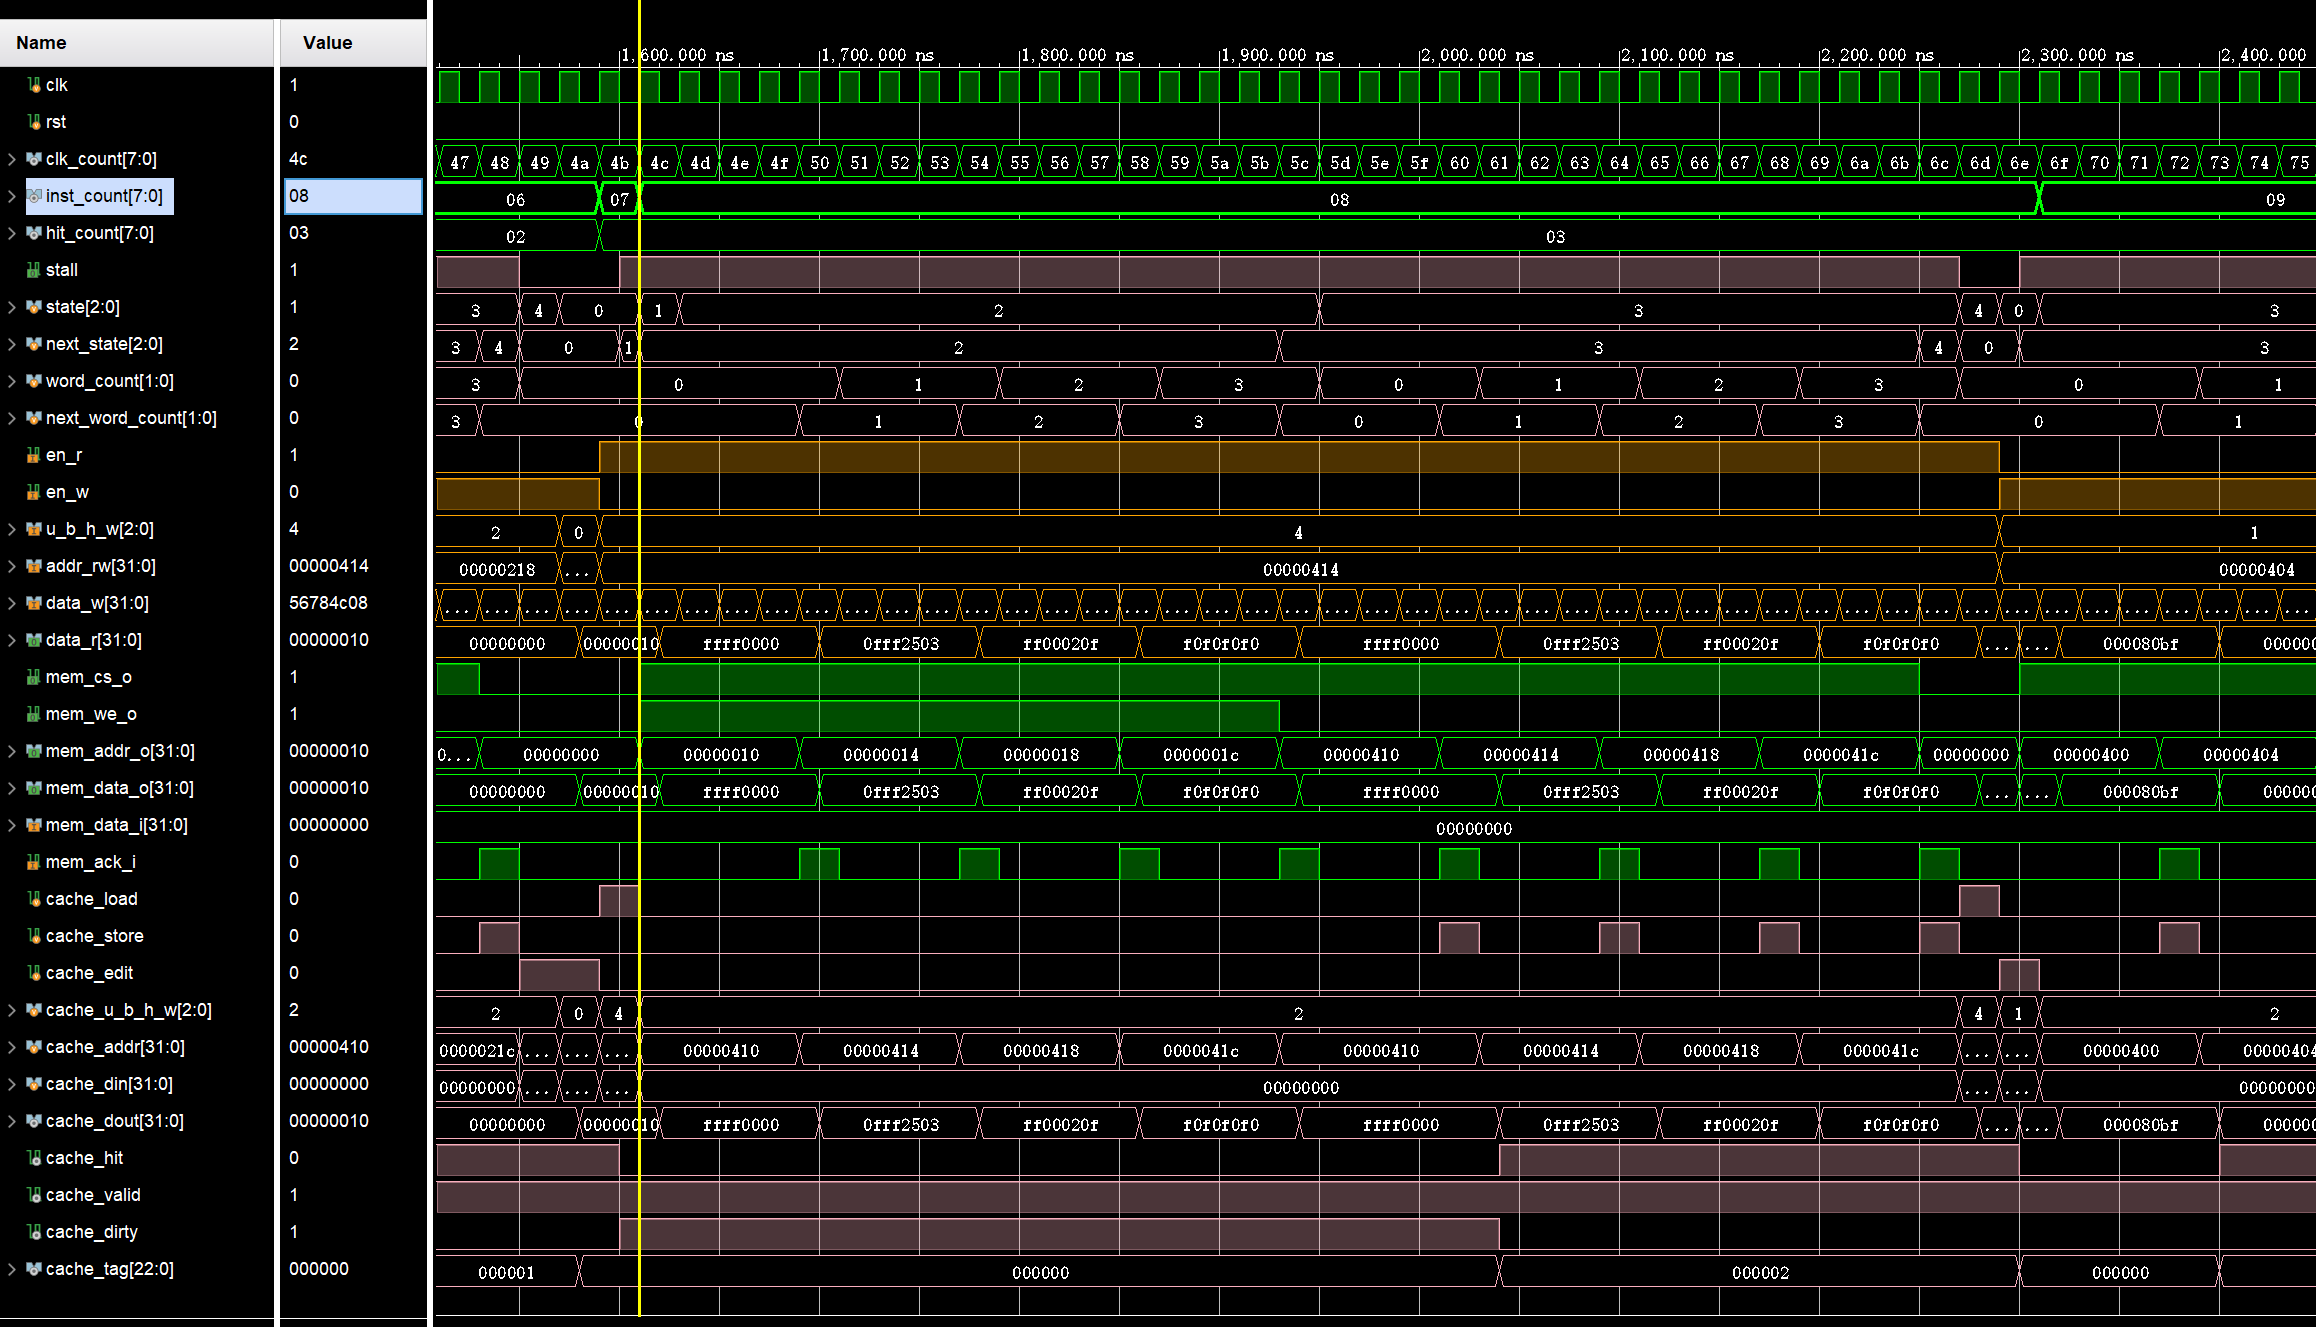
\includegraphics[width=1\textwidth]{images/cache_miss_dirty.png}
        \caption{Cache miss + dirty 仿真结果}
        \label{fig:cache_miss_dirty}
    \end{figure}
    当 cache miss 且 dirty 时,状态机的状态变化如下:\par
    初始状态为 S\_IDLE,接收到访存请求后(1个周期),进入 S\_PRE\_BACK 状态(1个周期),\par
    接着进入 S\_BACK 状态,依次完成对 4 个 word 的写回操作(16个周期),\par
    然后进入 S\_FILL 状态,依次完成对 4 个 word 的填充操作(16个周期),\par
    最后进入 S\_WAIT 状态,完成之前由于 miss 而不能进行的 Cache 操作(1个周期),\par
    然后回到 S\_IDLE 状态,完成读写操作。\par
    一共需要 35 个时钟周期。\par

\end{enumerate}

\newpage
\subsection{在本次实验中,Cache 采取的是 2 路组相联,在实现 LRU 替换的时候,每一个 set 需要用多少 bit 来用于真正的 LRU 替换实现?}
在 cache 模块的实现中,LRU 相关定义如下:\par
\begin{lstlisting}[language=Verilog]
    reg [ELEMENT_NUM-1:0] inner_recent = 0; // for LRU

    assign recent1 = inner_recent[addr_element1];
    assign recent2 = inner_recent[addr_element2]; 

    ...
    valid <= recent1 ? valid2 : valid1;
    dirty <= recent1 ? dirty2 : dirty1;
    tag <= recent1 ? tag2 : tag1;
\end{lstlisting}
可见,在 2 路组相联的情况下,每一个 set 只需要 1 bit 来表示 LRU 替换策略。\par

\end{document}